\chapter{Imbalance Detection Algorithm} % Chapter title

\todo{describe LifeLine system.}

\label{ch_detection_algorithm}

%----------------------------------------------------------------------------------------
%	Overview
%----------------------------------------------------------------------------------------
\section{Overview}
A rotor imbalance can causes problems and failures with the turbine, so it is important to detect the ``state" of the turbine using some measured input.  Turbine dynamics are complicated, vary between different systems and can be dependent on many variables.  An effective way to develop a model that is optimized for each different turbine is to use machine learning (ML).  Machine learning is the study of algorithms that build mathematical models to perform specific tasks without explicit instructions.

\subsection{Machine learning background}
The 2 main types of machine learning algorithms are supervised and unsupervised learning.  Supervised algorithms assume that each data set is assigned an output, while unsupervised algorithms take a data set of only inputs and attempt to create groups and classes from the input data.  For this application, each measurement data set from the turbine will be manually labeled as ``good" or ``bad" (or as ``balanced"/``unbalanced"), which is a type of supervised learning.

Machine learning algorithms also fall into the ``regression" or ``classification" categories.  Regression algorithms are used if the output is a continuous function, while classification algorithms are used if the output falls into distinct classes.  The output for the turbine detection algorithm is the state of the turbine (balanced/imbalanced), which is a discrete classification.

Knowing that the ML algorithm must be a classification, supervised model, the specific algorithm choice can be narrowed down.  Some of the common algorithms are logistic regression (this can be used as a classification algorithm even though it is called ``regression"), k-nearest neighbor, and neural networks.  This paper will analyze each of these models and apply them to the experimental turbine data.

\section{The training data}
Typically, it is common for machine learning algorithms to split the data into test and training sub groups.  This allows the accuracy of the models to be trained and evaluated on different data sets.  The input data for the turbine is a 256-point frequency spectrum of the acceleration data at the top of the tower.  Figure \ref{fig:LL_spectrogram} shows a spectrogram of the measured acceleration data.  A spectrogram is a way to visualize frequency data over time in a 2-dimensional figure, where the magnitudes of each frequency component are represented by a different color.  The spectrogram shows that there is a strong frequency component at about 2.4 Hz (the rotor frequency) that is constant throughout most of the operation.

\begin{figure}
	\centering
	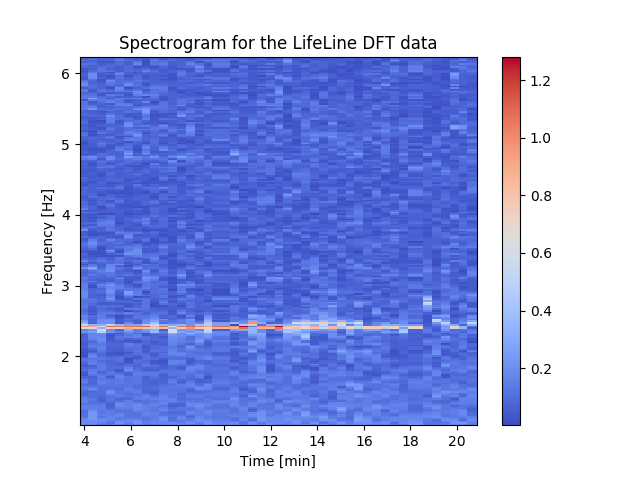
\includegraphics[scale=0.8]{LL_spectrogram}
	\decoRule
	\caption{This figure shows the spectrogram of the tower accelerations.}
	\label{fig:LL_spectrogram}
\end{figure}

Currently, only a single set of about 100 training examples exists.  The data can be separated into 2 classes; however, there is no information about which is the \textit{balanced} and \textit{imbalanced} classes.  To properly train the machine learning models, more data is required.  Despite the lack of available data, this paper will discuss the methods and implementations of each algorithm using the limited data set.


\section{K-Nearest Neighbor algorithm}
\section{About the algorithm}
The k-nearest neighbor (KNN) algorithm is one of the simplest models, but can be the most accurate and powerful when dealing with fairly small data sets.  This model essentially ``memorizes" the training data and plots the points in $n$-dimensional space.  The classification of a new point is calculated based on the distances between the new point and the training points.  For example, Figure \ref{fig:knn_visualization} shows a visualization of the classification process for a 2-class system.  Since this algorithm uses all of the training data in memory, it becomes very slow with many inputs, and many training data sets.  The example in Figure \ref{fig:knn_visualization} is a 2-dimensional problem (only 2 inputs) with only a few data points, so the KNN algorithm works very well.


\begin{figure}
	\centering
	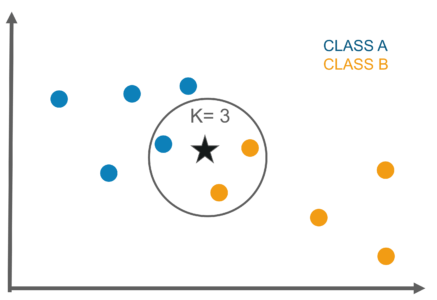
\includegraphics[scale=0.4]{knn_visualization}
	\decoRule
	\caption{A visualization of the KNN algorithm \cite{knn_python}.  The training data for a 2-class problem with 2 inputs is shown as blue and orange dots.  For $K=3$, a circle is drawn around the new point (star) until 3 training data points fall within the circle.  The classification of the new point is then determined by the majority of the points inside the circle.  In this case, there are more \textit{Class B} points than \textit{Class A} points, so the new point (star) will be classified as \textit{Class B}.}
	\label{fig:knn_visualization}
\end{figure}

The K-NN algorithm uses a "majority voting" method where the Euclidian distance between all the training data points and the test data is calculated.  This model assumes there is a relatively equal amount of balanced rotor experimental data and imbalanced experimental rotor data, which means the sample weighting can be uniform.  If there is a much higher frequency class (for example, much more balanced experimental data), this class will tend to dominate the calculations regardless of the actual class of the test data.

The number of neighbors, $k$, is chosen to be 5 for this algorithm (using trial and error).  A larger value of $k$ will reduce the classification noise, but the boundaries are much more general and not as tuned to the training data.  A lower value of $k$ will match the model very closely to the training data, but may add noise into the classification process.

The Euclidean distance is simply the distance between the data points.  This equation is shown below:

\begin{equation}
	d = \sqrt{\sum{\left(x_{i,a}-x_{j,a}\right)^2}}
\end{equation}

\subsection{Choosing the data}
The KNN algorithm works well on small data sets, so the DFT data should be pre-processed and cut down to a smaller, 2-dimensional data set.  Based on a simplified dynamic model of the turbine tower, a rotor imbalance will cause a high frequency excitation at the rotor frequency.  Using the maximum frequency component of the experimental DFT data and the corresponding frequency is a good way to capture enough information about the tower, while also reducing the data set from 256 input points to only 2 input points.

Figure \ref{fig:single_dft} shows the frequency spectrum from a single DFT calculation.  To convert this data into 2-dimensional data for the KNN algorithm, the peak value and corresponding frequency are extracted from this data.  For example, Figure \ref{fig:single_dft} would produce a 2-dimensional data set as shown in Equation \ref{eq:2d_data}.
\begin{equation} \label{eq:2d_data}
	[frequency, amplitude, class] = [2.3, 1.0, Class A]
\end{equation}

\begin{figure}
	\centering
	\includegraphics[scale=0.4]{single_dft}
	\decoRule
	\caption{This figure shows a single DFT result (a single column from Figure \ref{fig:LL_spectrogram}).}
	\label{fig:single_dft}
\end{figure}

By converting the entire data set for all training examples into 2-dimensional data, the data in Figure \ref{fig:LL_spectrogram} can be represented as the data in Figure \ref{fig:max_balanced_freq_mag}.

\begin{figure}
	\centering
	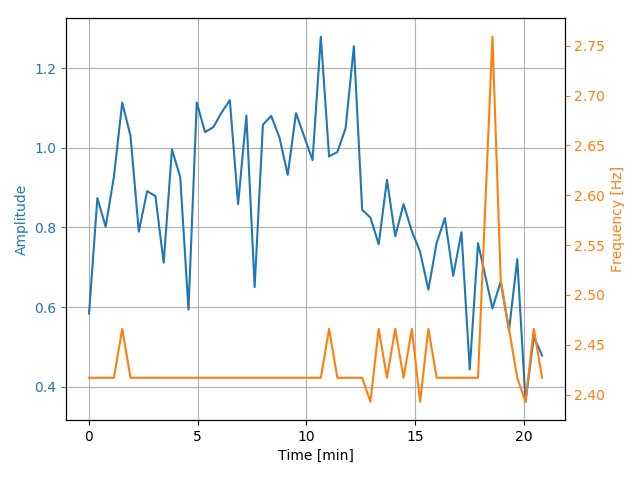
\includegraphics[scale=0.8]{max_balanced_freq_mag}
	\decoRule
	\caption{This figure shows a the 2-dimensional data used as an input to the KNN classification algorithm.}
	\label{fig:max_balanced_freq_mag}
\end{figure}


\subsection{Algorithm Results}
To apply the algorithm, the data is converted into short lists containing a maximum amplitude, a corresponding frequency value, and the known class (Equation \ref{eq:2d_data}). For this test, there are 55 experimental DFT results for \textit{Class A} and 55 experimental DFT results for \textit{Class B}. 

Training the KNN model is extremely fast and only involves storing all of the training data in memory.  When the algorithm is applied to new test examples, the results can be visualized in a confusion matrix \cite{confusion_matrix} as shown in Equation \ref{eq:knn_confusion_matrix}.  A confusion matrix is a common tool used to describe the performance of a classification algorithm.  This is an $n$ by $n$ matrix (where $n$ is the number of classes) that essentially shows the amount of correct and incorrect guesses for each class.  Table \ref{t:confusion_matrix_ex} shows a labeled version of the confusion matrix shown in Equation \ref{eq:knn_confusion_matrix}.

\begin{equation} \label{eq:knn_confusion_matrix}
C_{confusion} = 
\begin{bmatrix}
	12 & 1 \\
	3 & 6
\end{bmatrix}
\end{equation}

\begin{table}[]
\centering
\caption{An example of the terminology for the confusion matrix in Equation \ref{eq:knn_confusion_matrix}. \textit{Class A} and \textit{Class B} represent the different classes of data.  These can be related to a \textit{balanced} and \textit{imbalanced} rotor with proper data set labels.}
\label{t:confusion_matrix_ex}
\vspace*{0.2in}
\begin{tabular}{lllll}
\cline{2-3}
\multicolumn{1}{l|}{}                      & \multicolumn{1}{l|}{\textbf{Predicted Class A}} & \multicolumn{1}{l|}{\textbf{Predicted Class B}} &  &  \\ \cline{1-3}
\multicolumn{1}{|l|}{\textbf{Actual Class A}}  & \multicolumn{1}{l|}{12}                     & \multicolumn{1}{l|}{1}                       &  &  \\ \cline{1-3}
\multicolumn{1}{|l|}{\textbf{Actual Class B}} & \multicolumn{1}{l|}{3}                      & \multicolumn{1}{l|}{6}                       &  &  \\ \cline{1-3}
                                           &                                             &                                              &  & 
\end{tabular}
\end{table}


\begin{figure}
	\centering
	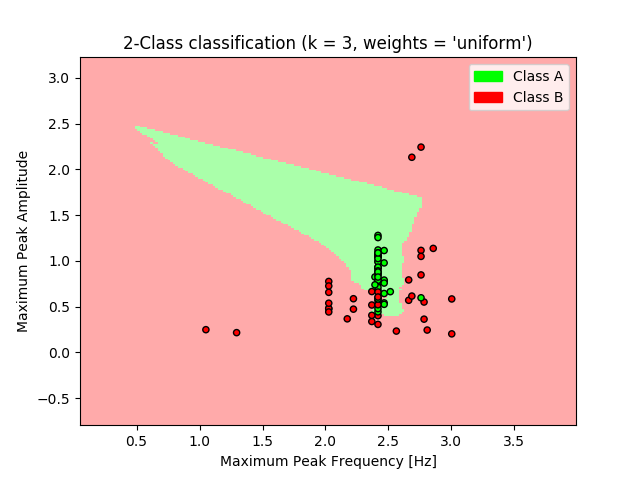
\includegraphics[scale=0.8]{knn_decision_boundary_k_3}
	\decoRule
	\caption{This figure shows the classification boundary for the KNN algorithm with $K=3$ for all of the training data.}
	\label{fig:knn_decision_boundary_k_3}
\end{figure}

A nice way to visualize the results of the classification algorithm with 2-dimensional inputs is to create a decision boundary plot.  A decision boundary is the area in space where the algorithm switches to a different classification.  Figure \ref{fig:knn_decision_boundary_k_3} shows the classification boundary for the KNN algorithm with $K=3$.

Initially, the balanced and imbalanced classes were expected to be easily distinguishable from each other.  Despite not having accurate labels of the experimental data, the imbalanced rotor data was expected to have much higher amplitudes at the rotor frequency; however, from Figure \ref{fig:knn_decision_boundary_k_3}, there isn't a significant difference between the amplitudes of the 2 data classes.

One observation that can be made from the data shown in Figure \ref{fig:knn_decision_boundary_k_3} is that the Class A data seems to have more frequency stability.  The Class A data has a constant frequency of about 2.5 Hz, while the Class B data has varying frequencies.  There is not enough data to make any hard conclusions, but this variance could be caused by either wind speed fluctuations or an actual property of the imbalance.  It is possible that an imbalance in the rotor could cause more variations in rotor speed, despite not having significant amplitude differences.  However, until the data can be accurately labeled, or more experimental data is collected, these classes should remain Class A and Class B to avoid any incorrect assumptions about the rotor imbalance.

\section{Logistic Regression}
\subsection{About the algorithm}
Logistic regression (LR) is a modified version of linear regression that is adapted for classification problems.  Logistic regression minimizes the squared error of a linear combination of the input parameters when passed through a sigmoid function.  To fully understand logistic regression, a brief background of linear regression is required. 

Linear regression is the process of minimizing the least squares cost of a data set with a linear function.  This is a commonly utilized method in curve fitting, but can also be applied to very high order systems.  Mathematically, this means minimizing the cost function shown in Equation \ref{eq:linear_regression_cost_fun}.  The hypothesis is the linear curve fit shown in Equation \ref{eq:linear_regression_hypothesis}.
\begin{align}
	J\left(\vec{\theta}\right) &= \frac{1}{2m} \sum_{i=1}^{m}{\left(h_{\theta}(x_i) - y_i\right)^2} \label{eq:linear_regression_cost_fun} \\
	h_{\theta}(x) &= \mat{x} \cdot \vec{\theta}^T\label{eq:linear_regression_hypothesis} \\
	\vec{\theta} &= [\theta_1, \theta_2, \theta_3, \hdots, \theta_n]
\end{align}

$n$ is the number of parameters (or features) in the input, $\mat{x}$.  $m$ is the number of training examples, which means $\mat{x}$ is of size $[m, n]$ and $\vec{\theta}$ is a vector with $n$ elements.

In order to apply linear regression to classification problems, the sigmoid function is applied to the linear regression hypothesis ($h_{\theta}$).  The sigmoid function is defined in Equation \ref{eq:sigmoid_function} and is visually shown in Figure \ref{fig:sigmoid_plot}.  The sigmoid function is designed to map an input to a value between 0 and 1, which represents the probability that the input is of a certain class.  This sigmoid function is what enables logistic regression to calculate binary outputs.
\begin{equation} \label{eq:sigmoid_function}
	g(z) = \frac{1}{1+e^{-z}}
\end{equation}

\begin{figure}
	\centering
	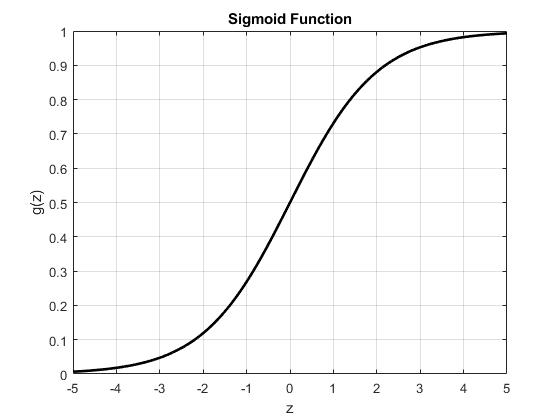
\includegraphics[scale=0.6]{sigmoid_plot}
	\decoRule
	\caption{This figure shows the sigmoid function plot.}
	\label{fig:sigmoid_plot}
\end{figure}

This new hypothesis function (Equation \ref{eq:logistic_regression_hypothesis}) produces a new cost function, shown in Equation \ref{eq:logistic_regression_cost}.
\begin{align}
	J(\theta) &= \frac{1}{m} \sum_{i=1}^{m}{\left[y_i \ln({h_{\theta}(x_i))} + (1-y_i) \ln{(1-h_{\theta}}) \right]}  \label{eq:logistic_regression_cost} \\
	h_{\theta} &= g(\mat{x} \cdot \vec{\theta}^T) = \frac{1}{1+e^{-(\mat{x} \cdot \vec{\theta}^T)}} \label{eq:logistic_regression_hypothesis}
\end{align}

The goal of logistic regression is to create a model that best fits the experimental training data by optimizing the parameters $\vec{\theta}$ to minimize the cost function, $J(\theta)$.  To do this, the gradient descent method is used \cite{gradient_descent}.  To  perform gradient descent, both the cost function and the gradient function of $\vec{\theta}$ are required.  The gradient can be numerically calculated using the finite difference method \cite{finite_difference_method}; however, this is much more computationally intensive than directly calculating the gradient analytically.  The derivative of the sigmoid function is shown in Equation \ref{eq:sigmoid_derivative}.  This produces a simple equation for the gradient of the cost function, which is shown in Equation \ref{eq:logistic_regression_gradient}.
\begin{align}
	g\prime(z) &= g(z) (1-g(z)) \label{eq:sigmoid_derivative} \\
	\frac{\partial J(\theta)}{\partial \theta_j} &= \frac{1}{m} \sum_{i=1}^{m}{\left(h_{\theta}(x_i) - y(i)\right) x_{j,i}} \label{eq:logistic_regression_gradient}
\end{align}

$h_{\theta}$ is defined in Equation \ref{eq:logistic_regression_hypothesis} and $g(z)$ is defined in Equation \ref{eq:logistic_regression_cost}.  In other words, Equation \ref{eq:logistic_regression_gradient} represents an average of $(h-y)x$ for every training example and calculated with respect to each $\theta$ parameter ($j$ is the number of parameters in the model).

%
%The filtered data produces a much more accurate detection model because much of the time-dependent noise is suppressed.  It is difficult to draw conclusive results from these test results, since there are only 55 sets of balanced and imbalanced data.  80 percent of this data is used to train the detection algorithm, while the remaining 20 percent is used to perform the verification testing shown in the confusion matrices and accuracy results.
%
%Both the amplitude and frequency values are important in detecting an imbalance in the turbine rotor.  An imbalance will cause overall higher acceleration amplitudes, but will also cause a larger variation in rotor speeds.  As shown in Figure  \ref{fig:classification_boundaries_filter}, the imbalanced data has large variations in both the maximum amplitude and frequency of the LifeLine DFT data.  When there is an imbalance in the rotor, the closed-loop transfer function of the changes, causing error in the tuned rotor speed controller parameters.  This causes some instability in the controller that is identified by the DFT results of the LifeLine module.
%
%Additionally, this algorithm can also be made more robust by looking for 10 or more positive imbalance detections in a row before flagging an alert.  This will remove any false positives that could shut the turbine down unintentionally.
%
%\begin{figure}
%	\centering
%	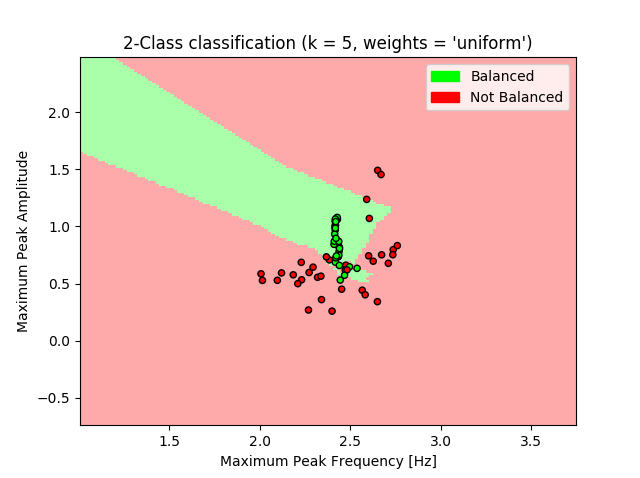
\includegraphics[scale=0.8]{classification_boundaries_filter}
%	\decoRule
%	\caption{The classification boundaries for test and training data that \textit{is} filtered.}
%	\label{fig:classification_boundaries_filter}
%\end{figure}
%
%
%
%%----------------------------------------------------------------------------------------
%%	SECTION 2
%%----------------------------------------------------------------------------------------
%\section{Detecting an imbalance}
%
%\todo{More explanation about the types of machine learning algorithms.  Explain the strengths and weaknesses of each method and include some background on machine learning.  Start with an explanation about the comparison between machine learning and linear regression.}
%
%\subsection{Selecting a classification algorithm}
%The crude and simple way to determine if there is an imbalance is to use a threshold criterion for the magnitude of the largest frequency component.  This method does not utilize the frequency values that correspond to each magnitude.  Since the rotor RPM is a range (not a constant value), it is likely that the magnitude will be slightly higher if the turbine is running faster and slightly lower if the turbine is running slower.  Additionally, the threshold method does not adapt the algorithm to patterns and new information gained from more data.
%
%This is a standard "classification" problem, where the algorithm needs to classify the state of the turbine as \textit{balanced} or \textit{not balanced}.  With the modern availability of computational power, classification algorithms tend to fall under the "machine learning" category.  These algorithms consist of a model that adapts to training data in order to minimize the error.  A few of the common models include Logistic Regression (LR), Linear Discriminant Analysis (LDA), K-Neighbors Classifier (KNC), Decision Tree Classifier (DNC), Gaussian Naive Bayes (GNB), and Support Vector Classification (SVC).
%
%The Logistic Regression model is commonly used to estimate discrete values (0/1 or false/true) and uses the logistic curve equation as the probability model.  The Linear Discriminant Analysis model address many of the shortcomings of the Logistic Regression model, such as multi-class classification and a higher stability.  Because the turbine classification problem only has 2 classes, this model is not likely to be the most optimal.
%
%The K-Neighbors Classifier model is one of the simplest models, but can be the most accurate and powerful when dealing with fairly small datasets.  This model essentially "memorizes" the training data and plots the points in $n$-dimensional space.  The classification of the new point is calculated based on the distances between the new point and the training points.  This model is likely to be an accurate algorithm for the turbine problem.
%
%Decision Tree Classification relies on the ability to split the data set into binary categories and subcategories, where the algorithm can follow yes/no decisions to lead to the correct class.
%
%The Gaussian Naive Bayes model is a statistics based model that modifies a prior belief bell curve based on the training data.  This is a statistical method of classifying data where the data set statistics are constantly updated with new data (as opposed to static models, such as mean, median, and standard deviation classification).
%
%The Support Vector Classification model creates a $n$-dimensional space where the training data points are divided by a clear gap that is as wide as possible.
%
%To compare the listed classification models against each other, the accuracy of each model is plotted using the same training and test data.  Figure \ref{fig:algorithm_comparison} shows that the K-Neighbors Classification algorithm has one of the highest mean accuracy ratings with the smallest variation is accuracy scores.  This is also the simplest to design and implement, which makes it an ideal choice for the imbalance detection algorithm that may need to run on a microprocessor attached to the turbine tower.
%
%\begin{figure}
%	\centering
%	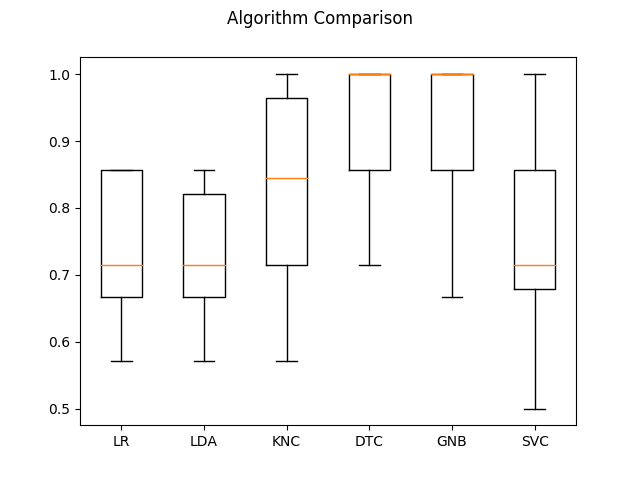
\includegraphics[scale=0.8]{algorithm_comparison}
%	\decoRule
%	\caption{A statistical comparison of different classification algorithms.  The algorithms compared are: Logistic Regression (LR), Linear Discriminant Analysis (LDA), K-Neighbors Classifier (KNC), Decision Tree Classifier (DNC), Gaussian Naive Bayes (GNB), and Support Vector Classification (SVC). \todo{Add axis label}}
%	\label{fig:algorithm_comparison}
%\end{figure}
%
%\subsection{Applying the K-Neighbors Classification Algorithm}
%\subsubsection{About the algorithm}
%The K-Neighbors Classifier (also known as the K-Nearest Neighbors Classifier or K-NN Classifier) is a type of "lazy learning" \cite{k_NN_algorithm}, which means it memorizes the training data and uses it to calculate the test data classification.  This results in a very short training time, but a longer calculation time curing the classification process.
%
%
%The K-NN algorithm uses a "majority voting" method where the Euclidian distance between all the training data points and the test data is calculated.  This model assumes there is a relatively equal amount of balanced rotor experimental data and imbalanced experimental rotor data, which means the sample weighting can be uniform.  If there is a much higher frequency class (for example, much more balanced experimental data), this class will tend to dominate the calculations regardless of the actual class of the test data.
%
%The number of neighbors, $k$, is chosen to be 5 for this algorithm (using trial and error).  A larger value of $k$ will reduce the classification noise, but the boundaries are much more general and not as tuned to the training data.  A lower value of $k$ will match the model very closely to the training data, but may add noise into the classification process.
%
%The Euclidean distance is simply the distance between the data points.  This equation is shown below:
%
%\begin{equation}
%	d = \sqrt{\sum{\left(x_{i,a}-x_{j,a}\right)^2}}
%\end{equation}
%
%\subsubsection{Algorithm Results}
%To apply the algorithm, the data is converted into short lists containing a maximum amplitude, a corresponding frequency value, and the known class. For this test, there are 55 experimental DFT results for a balanced rotor and 55 experimental DFT results for an imbalanced rotor.  Applying the algorithm on raw DFT data produces the classification boundary plot shown in Figure \ref{fig:classification_boundaries_no_filter}.  Using unfiltered data is slightly faster (there is no filter lag), but the accuracy is significantly reduces.  It is much more accurate to filter the data first, if the lag is an acceptable consequence.  The unfiltered data produces an accuracy of about 86 percent with a confusion matrix:
%
%\todo{Explain what a confusion matrix is.}
%
%\begin{equation}
%C_{confusion} = 
%\begin{bmatrix}
%	13 & 0 \\
%	3 & 6
%\end{bmatrix}
%\end{equation}
%
%\begin{figure}
%	\centering
%	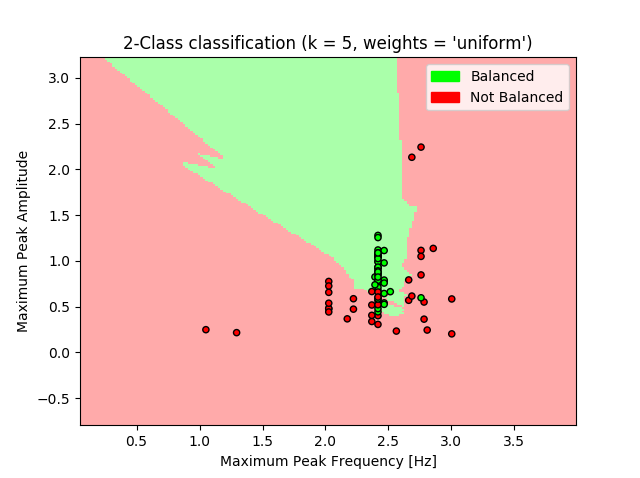
\includegraphics[scale=0.8]{classification_boundaries_no_filter}
%	\decoRule
%	\caption{The classification boundaries for test and training data that is not filtered.}
%	\label{fig:classification_boundaries_no_filter}
%\end{figure}
%
%Figure \ref{fig:classification_boundaries_filter} shows the classification boundaries with data filtered using an IIR filter.  A clear trend can be seen in this data, with distinct class boundaries.  This produces an accuracy of 94 percent with a confusion matrix:
%
%\begin{equation}
%C_{confusion,filtered} = 
%\begin{bmatrix}
%	6 & 1 \\
%	0 & 11
%\end{bmatrix}
%\end{equation}
%
%The filtered data produces a much more accurate detection model because much of the time-dependent noise is suppressed.  It is difficult to draw conclusive results from these test results, since there are only 55 sets of balanced and imbalanced data.  80 percent of this data is used to train the detection algorithm, while the remaining 20 percent is used to perform the verification testing shown in the confusion matrices and accuracy results.
%
%Both the amplitude and frequency values are important in detecting an imbalance in the turbine rotor.  An imbalance will cause overall higher acceleration amplitudes, but will also cause a larger variation in rotor speeds.  As shown in Figure  \ref{fig:classification_boundaries_filter}, the imbalanced data has large variations in both the maximum amplitude and frequency of the LifeLine DFT data.  When there is an imbalance in the rotor, the closed-loop transfer function of the changes, causing error in the tuned rotor speed controller parameters.  This causes some instability in the controller that is identified by the DFT results of the LifeLine module.
%
%Additionally, this algorithm can also be made more robust by looking for 10 or more positive imbalance detections in a row before flagging an alert.  This will remove any false positives that could shut the turbine down unintentionally.
%
%\begin{figure}
%	\centering
%	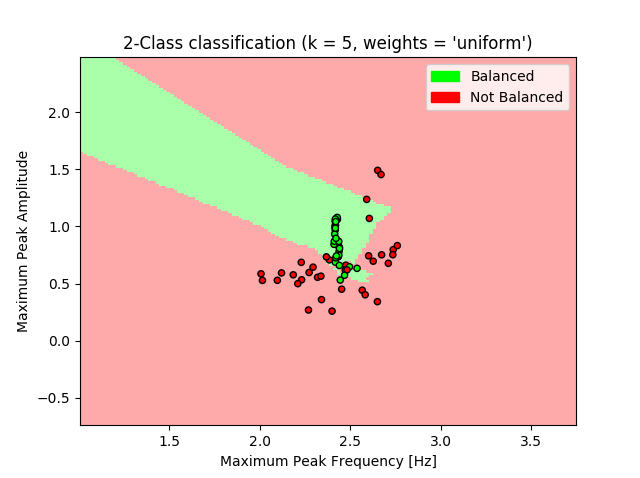
\includegraphics[scale=0.8]{classification_boundaries_filter}
%	\decoRule
%	\caption{The classification boundaries for test and training data that \textit{is} filtered.}
%	\label{fig:classification_boundaries_filter}
%\end{figure}
%
%
%%----------------------------------------------------------------------------------------
%%	SECTION 3
%%----------------------------------------------------------------------------------------
%\section{Analyzing the Detection Algorithm}
%\subsection{Using Different Parameters}
%The main parameters to tune for the detection model are $k$ and the weighting.  In the KNN algorithm, the classification decision is based on the weighted vote from $k$ neighboring samples.  This means that a larger $k$ value will include more data in each decision, but may be lest accurate.  A smaller $k$ value will create tight classification boundaries, but could be prone to over-fitting.  Figure \ref{fig:classification_k_20_uniform} and Figure \ref{fig:classification_k_2_uniform} show the effect of changing the $k$ value on the classification boundaries.
%
%\begin{figure}
%	\centering
%	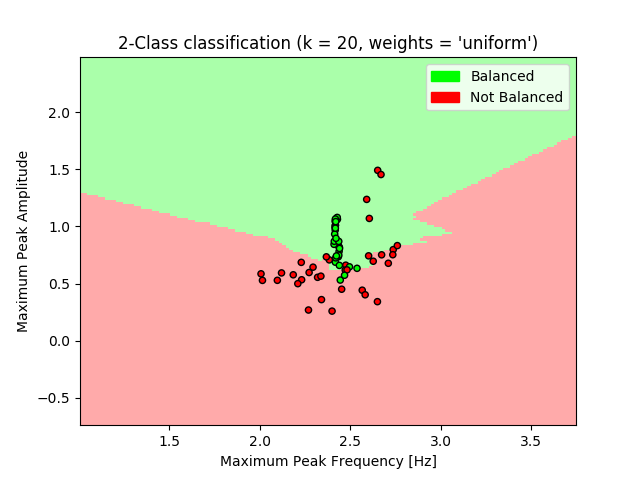
\includegraphics[scale=0.8]{classification_k_20_uniform}
%	\decoRule
%	\caption{The classification boundaries with $k=20$ and uniform weighting.}
%	\label{fig:classification_k_20_uniform}
%\end{figure}
%
%\begin{figure}
%	\centering
%	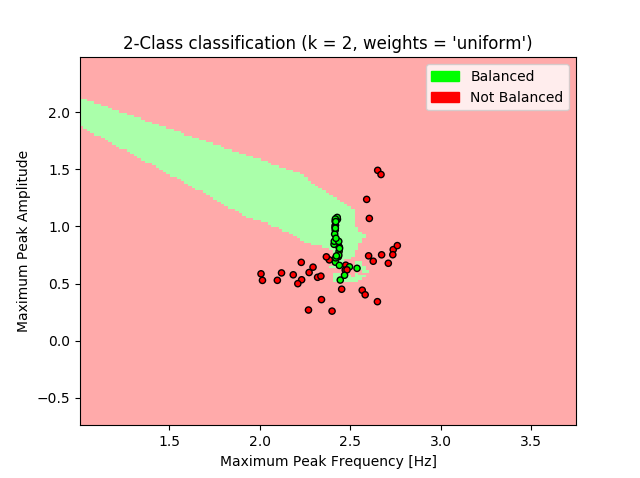
\includegraphics[scale=0.8]{classification_k_2_uniform}
%	\decoRule
%	\caption{The classification boundaries with $k=2$ and uniform weighting.}
%	\label{fig:classification_k_2_uniform}
%\end{figure}
%
%\subsection{Potential Problems}
%One of the biggest problems with the KNN classification algorithm is the computational cost.  Because this is a "memory-based" model, the training data is essentially locked in memory and used to classify any new inputs.  By changing the model, the computational cost can be reduced; however, these are much more complicated to implement and not always as accurate.
%
%Additionally, the IIR filter has a fairly significant and nonlinear delay that increases near DC frequency components.  Faster filters can be used at the cost of accuracy because they will produce more noise or a more distorted signal.  For this application, it seems like accuracy is more important than speed, and the IIR filter parameters were designed around this idea.
%
%This detection algorithm is best developed with real experimental data, which means it requires actual data before it is of any use.  If a sufficient enough model is developed, the model can produce the test data to train the algorithm instead of collecting it in the field; however, this is likely to be less accurate.
%
%\subsection{Future Changes}
%
%\todo{Add a section about algorithm scalability and switching to a model-based machine learning algorithm (like a neural network) if many training sets are acquired.}
%
%One of the significant benefits with this algorithm is the flexibility.  It is very easy to add more data to improve the imbalance detection.  For example, in addition to peak frequency and magnitude, the wind speed and generator power can be included as parameters to improve the model.  With enough variables and experimental data, the model will become more accurate and robust (although it is difficult to visualize the classification space with orders higher than 2).
%
%In addition, the entire frequency spectrum can be used as an input to the algorithm (instead of just using the peak values), but the model becomes much more complex.  With a large amount of experimental data, the KNN model might need to be changed to a less computationally intensive model, such as a neural network.
%
%Just using a classification algorithm on raw data isn't always useful.  It is very important to properly choose a data processing methods, such as the IIR filter used in this paper.  Selecting the filter is just as important as choosing the model for this type of data.
%
%\todo{Add a section with conclusions, recommendations for future work, and methods for algorithm improvement.  Add code to a public repository.}
%
%
%
%
%






